\chapter{Testing}
\label{chap:testing}

This chapter outlines the process of testing with React.js and Go. The chapter will also cover the use of Postman for API testing and Chrome Developer Tools for debugging and testing in the browser.

\section{Unit Testing}
\label{testing:unit}

% add some context here (why am I testing, how does it fit into what the user expects)

For unit testing, two frameworks were used. For the Go/Gin backend, the built-in Go test framework was used. For the React.js front, the Jest testing framework was used. The respective plugins were installed in VS Code to allow for easy running and visualisation of the tests \see{fig:unit-tests}.

Multiple tests were written to test the API GET endpoints. The tests were run via the aforementioned VS Code plugin or the terminal using the command `\texttt{go test}'. Using mock data inputs, the tests were written to ensure that the correct JSON object was returned in the correct format to be exploited by the front end.

Testing React.js components was a more complex process than writing tests for vanilla JavaScript. As the tests were required to be on a component-level basis, snapshot testing was used to ensure that the components were rendered correctly. To create a snapshot test, all data required by the component was mocked, including required functions. These functions were mocked using `\texttt{jest.fn}', `\texttt{jest.spyOn}' and `\texttt{mockImplementation}'. MockImplementation was used to mock the ChartJs Chart function, to ensure that the ElevationChart snapshot test was consistent with the actual component. To run the tests, either the command `\texttt{npm test}' or the VS Code plugin was used to run the tests.

\begin{figure}[!ht]
    \centering
    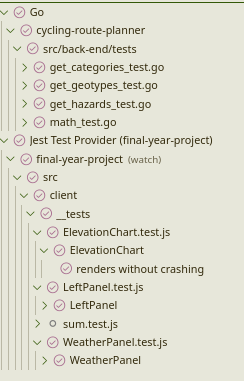
\includegraphics[width=150px]{figures/unit-tests.png}
    \caption{Unit Tests}
    \label{fig:unit-tests}
  \end{figure}

Manual unit tests were also conducted on the front end to ensure that the components behaved as expected. This was done by running the application and manually testing the components to ensure that they rendered correctly and that the data was displayed as expected \see{tab:unit-test-results}.

\begin{table}
\caption{Manual Unit Test Results}
\label{tab:unit-test-results}
\renewcommand{\arraystretch}{1.5} % Adjust the factor to suit your needs
\begin{tabular}{ p{1.85cm} p{10cm}  p{1.85cm} }
\hline
Test Case & Description & Pass?\\
\hline
 & \multicolumn{2}{p{11.85cm}}{\textbf{ElevationChart Component}}\\
01 & The component was tested to ensure that it renders correctly on load. & Y\\
02 & The component was tested to ensure that it renders correctly when changing the route. & Y\\
03 & The component was tested to ensure that it renders correctly when zooming into the chart. & Y\\
04 & The component was tested to ensure that it renders correctly when clicking reset zoom. & Y\\
\hline
 & \multicolumn{2}{p{11.85cm}}{\textbf{RoutingMachine Component}}\\
05 & The component was tested to ensure that it renders correctly on load. & Y\\
06 & The component was tested to ensure that it renders correctly when the waypoints are updated. & Y\\
07 & The component was tested to ensure that it renders correctly when the waypoints are dragged. & Y\\
08 & The component was tested to ensure that it renders correctly when the waypoints are removed. & Y\\
\hline
 & \multicolumn{2}{p{11.85cm}}{\textbf{WeatherPanel Component}}\\
09 & The component was tested to ensure that it renders correctly on load. & Y\\
10 & The component was tested to ensure that it renders correctly when the user shares their geolocation. & Y\\
\hline
 & \multicolumn{2}{p{11.85cm}}{\textbf{SharePanel Component}}\\
11 & The component was tested to ensure that it renders correctly on load. & Y\\
12 & The component was tested to ensure that it renders correctly when the share button is pressed. & Y\\
\hline
 & \multicolumn{2}{p{11.85cm}}{\textbf{RoutePreferencesPanel Component}}\\
13 & The component was tested to ensure that it renders correctly on load. & Y\\
14 & The component was tested to ensure that it renders correctly when the route preferences button is pressed. & Y\\
\end{tabular}
\end{table}

\section{Postman}
\label{testing:postman}

Postman was also used extensively through development to test the API. It was used to test the GET and POST endpoints to ensure that the correct data was being returned and that the correct data was being sent to the backend. In addition to testing the Go backend, Postman was also used to build and test API requests for Strava, Garmin Connect, Open Weather Map, Foursquare and the Here API. This was done to ensure that the API requests were being built correctly before being implemented into the artefact.

\section{Chrome Developer Tools}
\label{testing:chrome-dev}

The Chrome Developer Tools were also used to test the front end during development. The debugger was used to ensure that the JavaScript was running correctly and that the data was being passed correctly between the front and back end. Logs and breakpoints were also used to track the flow of data through the front end, ensuring that the state was being updated correctly and that the correct data was being passed to the components.